\documentclass[8pt]{article}
 
\usepackage[margin=.8in]{geometry} 
\usepackage{amsmath,amsthm,amssymb}
\usepackage{marvosym,enumerate,color,mathrsfs,graphicx,epstopdf}
%\usepackage{enumitem}
%\setenumerate{listparindent=\parindent}
\def\cc{\color{blue}}
%\usepackage[dvipsnames]{xcolor}
\usepackage[normalem]{ulem}
\usepackage{bm}
\usepackage{mathtools}
\usepackage{mathrsfs}
\usepackage{verbatim}
\usepackage{tikz}
\usepackage[utf8]{inputenc}
\usepackage{hyperref}
\usepackage{courier}
%\usepackage{fullpage}
\usepackage{graphicx}
\usepackage{float}
\hypersetup{
	%colorlinks,
	%citecolor=black,
	%filecolor=black,
	%linkcolor=blue,
	%urlcolor=black
}

%\setlength{\oddsidemargin}{-20pt}

%\setlength{\topmargin}{-50pt}
%\setlength{\footskip}{-50pt}


%\usepackage{multirow}

%Line Numbering
\usepackage[mathlines]{lineno}
%\linenumbers
 
\newcommand{\N}{\mathbb{N}}
\newcommand{\Z}{\mathbb{Z}}
\newcommand{\R}{\mathbb{R}}
\newcommand{\C}{\mathbb{C}}
\newcommand{\Q}{\mathbb{Q}}
%\newcommand{\dell}{\partial}
\newcommand{\abs}[1]{\left\lvert{#1}\right\rvert}
\newcommand{\dx}{\mathrm{d}x}
\newcommand{\M}{\mathscr{M}}
\newcommand{\E}{\mathscr{E}}
\newcommand{\B}{\mathscr{B}}
\newcommand{\scr}[1]{\mathscr{#1}}
\newcommand{\Ns}{\mathscr{N}}
\newcommand{\nm}{\mathrel{\unlhd}}
\newcommand{\stcomp}[1]{{#1}^{\mathsf{c}}}
\newcommand{\closure}[1]{\overline{#1}}
\newcommand{\diam}{\operatorname{diam}}
\newcommand{\dist}{\operatorname{dist}}
\newcommand{\sgn}{\operatorname{sgn}}
\newcommand{\norm}[1]{\left\lVert{#1}\right\rVert}
\newcommand{\LR}[1]{\left\langle{#1}\right\rangle}

\theoremstyle{definition}
\newtheorem{theorem}{Theorem}
\newtheorem*{theorem*}{Theorem}
\newtheorem{lemma}[theorem]{Lemma}
\newtheorem{proposition}[theorem]{Proposition}
\newtheorem*{proposition*}{Proposition}
\newtheorem{definition}[theorem]{Definition}
\newtheorem*{definition*}{Definition}
\newtheorem{remark}[theorem]{Remark(s)}
\newtheorem*{remark*}{Remark(s)}
\newtheorem{corollary}[theorem]{Corollary}
\newtheorem*{corollary*}{Corollary}
\newtheorem{innerexercise}{Exercise}
\newenvironment{exercise}[1]
  {\renewcommand\theinnerexercise{#1}\innerexercise}
  {\endinnerexercise}

% Upper and lower integrals
%\def\upint{\mathchoice%
%    {\mkern13mu\overline{\vphantom{\intop}\mkern7mu}\mkern-20mu}%
%    {\mkern7mu\overline{\vphantom{\intop}\mkern7mu}\mkern-14mu}%
%    {\mkern7mu\overline{\vphantom{\intop}\mkern7mu}\mkern-14mu}%
%    {\mkern7mu\overline{\vphantom{\intop}\mkern7mu}\mkern-14mu}%
%  \int}
%\def\lowint{\mkern3mu\underline{\vphantom{\intop}\mkern7mu}\mkern-10mu\int}

\title{Numerical Analysis -- Homework 6}
\author{James Diffenderfer}
\date{\today}

%%%%%%%%%%%%%%%%%%%%%%%%%%%%%%%%%%%%%%
\begin{document}

\maketitle
%\tableofcontents

%\newpage

\begin{exercise}{1}
Consider the perturbed Euler method 
\begin{align*}
u_0 &= \alpha + \delta_0 \\
u_{i+1} &= u_i + h f (u_i, t_i) + \delta_i
\end{align*}
with the $\delta_i$ representing round-off error. Show that for all $i$, $$|Y(t_i) - u_i| \leq \frac{1}{L} \left( \frac{hM}{2} + \frac{\delta}{h} \right) \left( e^{L(b-a)} - 1 \right) + | \delta_0| e^{L(b-a)},$$ where $\delta = \max | \delta_i |$ and $M = \max |Y''(t)|$, which we assume to be finite.
\end{exercise}

\begin{proof}
Note that I will often make use of the convention that $Y(t_i) = Y_i$. By Taylor's Theorem we have that there exists a $\xi_i \in [t_i, t_{n+1}]$ such that  
\begin{align*}
Y_{i+1} &= Y_i + Y'(t_i) h + \frac{h^2}{2} Y'' (\xi_i) = Y_i + h f(Y_i, t_i) + \frac{h^2}{2} Y'' (\xi_i).
\end{align*}
Defining $e_i = Y_i - u_i$, we now have that 
\begin{align}
|e_{i+1}| &= \left| \left[Y_i + h f(Y_i, t_i) + \frac{h^2}{2} Y'' (\xi_i) \right] - \left[ u_i + h f(u_i, t_i) + \delta_i \right] \right| \nonumber \\
&\leq \left|Y_i  - u_i \right| + h \left| f(Y_i, t_i)  - f(u_i, t_i) \right|+ \frac{h^2}{2} \left|Y'' (\xi_i) \right| + \left| \delta_i \right| \nonumber \\
&\leq \left| Y_i - u_i \right| + h L \left| Y_i - u_i \right|+ \frac{h^2 M}{2} + \delta \tag{Since $f$ is Lipschitz in y} \\
&= (1 + hL) \left| e_i \right| + \frac{h^2 M}{2} + \delta. \label{prob1}
\end{align}
Now recall the following lemma:
\begin{quote}
\emph{Lemma}: Suppose $s, t > 0$, $\{ a_i \}_{i = 0}^{k}$ with $a_0 \geq - \frac{t}{s}$ and $a_{i + 1} \leq (1 + s) a_i + t$. Then we have that $a_{i+1} \leq \left( e^{(1 + i)s} - 1 \right) \frac{t}{s} + a_0 e^{(1 + i)s}$.
\end{quote}
Accordingly, noting (\ref{prob1}), we let $s = hL$, $t = \frac{h^2 M}{2} + \delta$, and $a_0 = |\delta_0|$. Hence, we observe that (\ref{prob1}) satisfies the hypotheses of the lemma and since
\begin{align*}
(1+i)s &= (1+i)hL = (t_{i+1} - a)L \\
\frac{t}{s} &= \frac{\frac{h^2 M}{2} + \delta}{hL} = \frac{hM}{2L} + \frac{\delta}{hL} = \frac{1}{L} \left( \frac{hM}{2} + \frac{\delta}{h} \right)
\end{align*}
we conclude that 
\begin{align}
|e_{i+1}| &\leq \frac{1}{L} \left( \frac{hM}{2} + \frac{\delta}{h} \right) \left( e^{L(t_{i+1}-a)} - 1 \right) + | \delta_0| e^{L(t_{i+1}-a)}. \label{prob1.2}
\end{align}
Since the function $e^x$ is monotonically increasing, replacing $t_{i+1}$ by $b$ in (\ref{prob1.2}) yields the desired inequality which holds for all $i$.
\end{proof}

\newpage

\begin{exercise}{2}
With $\phi(w, t) = a f(w + bh, t + ch)$, find the values of the parameters $a$, $b$, $c$ so that the resulting one-step method 
\begin{align*}
w_0 &= \alpha \\
w_{i+1} &= w_i + h \phi(w_i, t_i)
\end{align*}
has local truncation error $O(h^2)$.
\end{exercise}

\begin{proof}
Note that in this problem I will be using the notations $f (t_i) = f(Y(t_i), t_i)$, and $f_Y (t_i) = \nabla_Y f(Y(t), t) \arrowvert_{t = t_i}$, and $f_t (t_i) = \nabla_t f(Y(t), t) \arrowvert_{t = t_i}$ to prevent the derivation from becoming too cluttered. Recall that the truncation error is given by 
\begin{align}
\tau_i (h) = \frac{Y_{i+1} - \left( Y_i + h \phi(Y_i, t_i) \right)}{h}. \label{prob2}
\end{align}
By Taylor's Theorem we have that 
\begin{align}
Y_{i+1} - Y_i &= h Y'(t_i) + \frac{h^2}{2} Y''(t_i) + O(h^3) \nonumber \\
&= h f(t_i) + \frac{h^2}{2} \left( f_Y (t_i) f (t_i) + f_t (t_i) \right) + O(h^3) \label{prob2.1}
\end{align}
and 
\begin{align}
\frac{1}{a} \phi (Y_i, t_i) &= f(Y_i + bh, t_i + ch) \nonumber \\
&= f(Y_i, t_i) + f_Y (t_i) bh + f_t (t_i) ch + O(h^2), \nonumber
\end{align}
which is equivalent to 
\begin{align}
\phi (Y_i, t_i) &= a f(t_i) + f_Y (t_i) abh + f_t (t_i) ach + O(h^2), \label{prob2.2}
\end{align}
since $a$ is a constant. Substituting (\ref{prob2.1}) and (\ref{prob2.2}) into (\ref{prob2}) yields
\begin{align}
\tau_i (h) &= \frac{h f(t_i) + \frac{h^2}{2} \left( f_Y (t_i) f (t_i) + f_t (t_i) \right) + O(h^3) - h \left( a f(t_i) + f_Y (t_i) abh + f_t (t_i) ach + O(h^2) \right)}{h} \nonumber \\
&= f(t_i) + \frac{h}{2} \left( f_Y (t_i) f (t_i) + f_t (t_i) \right) - \left( a f(Y_i, t_i) + f_Y (t_i) abh + f_t (t_i) ach \right) + O(h^2) \nonumber \\
&= (1-a) f(t_i) + h \left[ f_Y (t_i) \left( \frac{1}{2} f (t_i) - ab \right) + f_t (t_i) \left( \frac{1}{2} - ac \right) \right] + O(h^2). \label{prob2.3}
\end{align}
Hence, by taking $a = 1$, $b = \frac{1}{2} f(t_i)$, and $c = \frac{1}{2}$, the equation in (\ref{prob2.3}) simplifies to $$\tau_{i} (h) = O(h^2),$$ yielding the desired result.
\end{proof}

\newpage


\begin{exercise}{3}
Consider 
\begin{align}
y' = \frac{2}{t} y + t^2 e^t; \ \ t \in [1, 2]; \ \ y(1) = 0, \label{prob3}
\end{align}
which has solution $Y(t) = t^2 (e^t - e)$.
\begin{enumerate}
\item[(a)] Using the (unperturbed) Euler method error estimate, find the value of $h$ required to ensure that the Euler method solution $w_i$ of (\ref{prob3}) satisfies $|Y(t_i) - w_i| \leq 0.1$, for all $i$.
\item[(b)] Write a program to implement Euler's method and run it with the $h$ value computed in (a) (or more precisely, a value $h$ near it with $1/h = n \in \mathbb{N}$) and confirm that $|Y(t_i) - w_i| \leq 0.1$, for all $i$.
\item[(c)] Derive the Taylor method of order 3 for (\ref{prob3}).
\item[(d)] Write a program to implement this Taylor method and, by experimentation, find a value of $h$ which ensures that $|Y(t_i) - v_i| \leq 0.1$, for all $i$, where $v_i$ is the solution computed via Taylor's method.
\end{enumerate}
\end{exercise}

\begin{proof}[Proof for (a)]
In order to determine the required value of $h$ we need to determine $M = \max_{t \in [1, 2]} | Y''(t) |$ and the Lipschitz constant $L$. Accordingly, computing the derivatives we find that
\begin{align*}
Y' &= f(Y, t) = \frac{2}{t} Y + t^2 e^t \\
Y'' &= \frac{2}{t} Y' - \frac{2}{t^2} y + e^t (t^2 + 2t) = \frac{2}{t^2} Y + t^2 e^t + 4t e^t
\end{align*}
Subsituting the solution $Y(t) = t^2 (e^t - e)$ into the formula for $Y''$ yields
\begin{align*}
Y'' &= \frac{2}{t^2} (e^t - e) + t^2 e^t + 4t e^t.
\end{align*}
Hence $Y''(t)$ is increasing for $t \in [1, 2]$ so we have that $$M = \max_{t \in [1, 2]} | Y''(t) | = | Y'' (2) | = 2 (e^2 - e) + 4 e^2 + 8 e^2 = 2e (7e - 1).$$ Next, observing that 
\begin{align*}
|f(y,t) - f(w,t)| &= \left| \left( \frac{2}{t} y + t^2 e^t \right) - \left( \frac{2}{t} w + t^2 e^t \right) \right| \\
&= \frac{2}{|t|} |y - w|,
\end{align*}
we conclude that $|f(y,t) - f(w,t)| \leq 2 |y - w|$ for all $y, w$ and $t \in [1, 2]$. Hence, $L = 2$ is the Lipschitz constant. Using the formula for the error bound on Euler's method we have
\begin{align*}
\left| Y(t_i) - w_i \right| \leq \left( e^{(b-a)L} - 1 \right) \frac{hM}{2L} = (e^2 - 1) \frac{2e (7e - 1) h}{4} \leq 0.1.
\end{align*}
Solving for $h$ we obtain the inequality
\begin{align*}
h \leq \frac{4}{2e(7e - 1)(e^2 - 1)} \approx 0.0006387808944 \ \ \ \Longrightarrow \ \ \ 1566 \leq \frac{1}{h}.
\end{align*}
\end{proof}

\begin{proof}[Proof for (c)]
Computing derivatives we find that
\begin{align*}
Y' &= f(Y, t) = \frac{2}{t} Y + t^2 e^t \\
Y'' &= \frac{2}{t^2} Y + t^2 e^t + 4t e^t \\
Y''' &= e^t (t^2 + 6t + 6).
\end{align*}
The update for the 3rd order Taylor Method is given by 
\begin{align*}
w_{i+1} &= w_i + h f(w_i, t_i) + \frac{h^2}{2} \nabla_t f(w_i, t_i) + \frac{h^3}{6} \nabla_t^2 f(w_i, t_i) \\
&= w_i + h \left( \frac{2}{t_i} w_i + t_i^2 e^{t_i} \right) + h^2 \left( \frac{1}{t_i^2} w_i + \frac{1}{2} t_i^2 e^{t_i} + 2t_i e^t_i \right) + h^3 e^t_i \left( \frac{t_i^2}{6} + t_i + 1  \right).
\end{align*}
\end{proof}

\begin{proof}[Numerical Results]
The code for this assignment was written using python and is included on the final page of the assignment. Based on the work from part (a), the value of $h$ was set to $\frac{1}{1566}$ and yielded the error result $$\tt{|| Y - w ||_{inf} =  0.0234241022462},$$ as desired. For the third order Taylor's method, experimentation with various values of $h$ yielded that the largest value of $h$ for which $\| Y - w \|_{\infty} \leq 0.1$ was $h = 0.2$. In this instance, 
$$\tt{|| Y - w ||_{inf} =  0.0579913386802}.$$
\end{proof}


\end{document}

% Figure Stuff
\begin{figure}[H]
	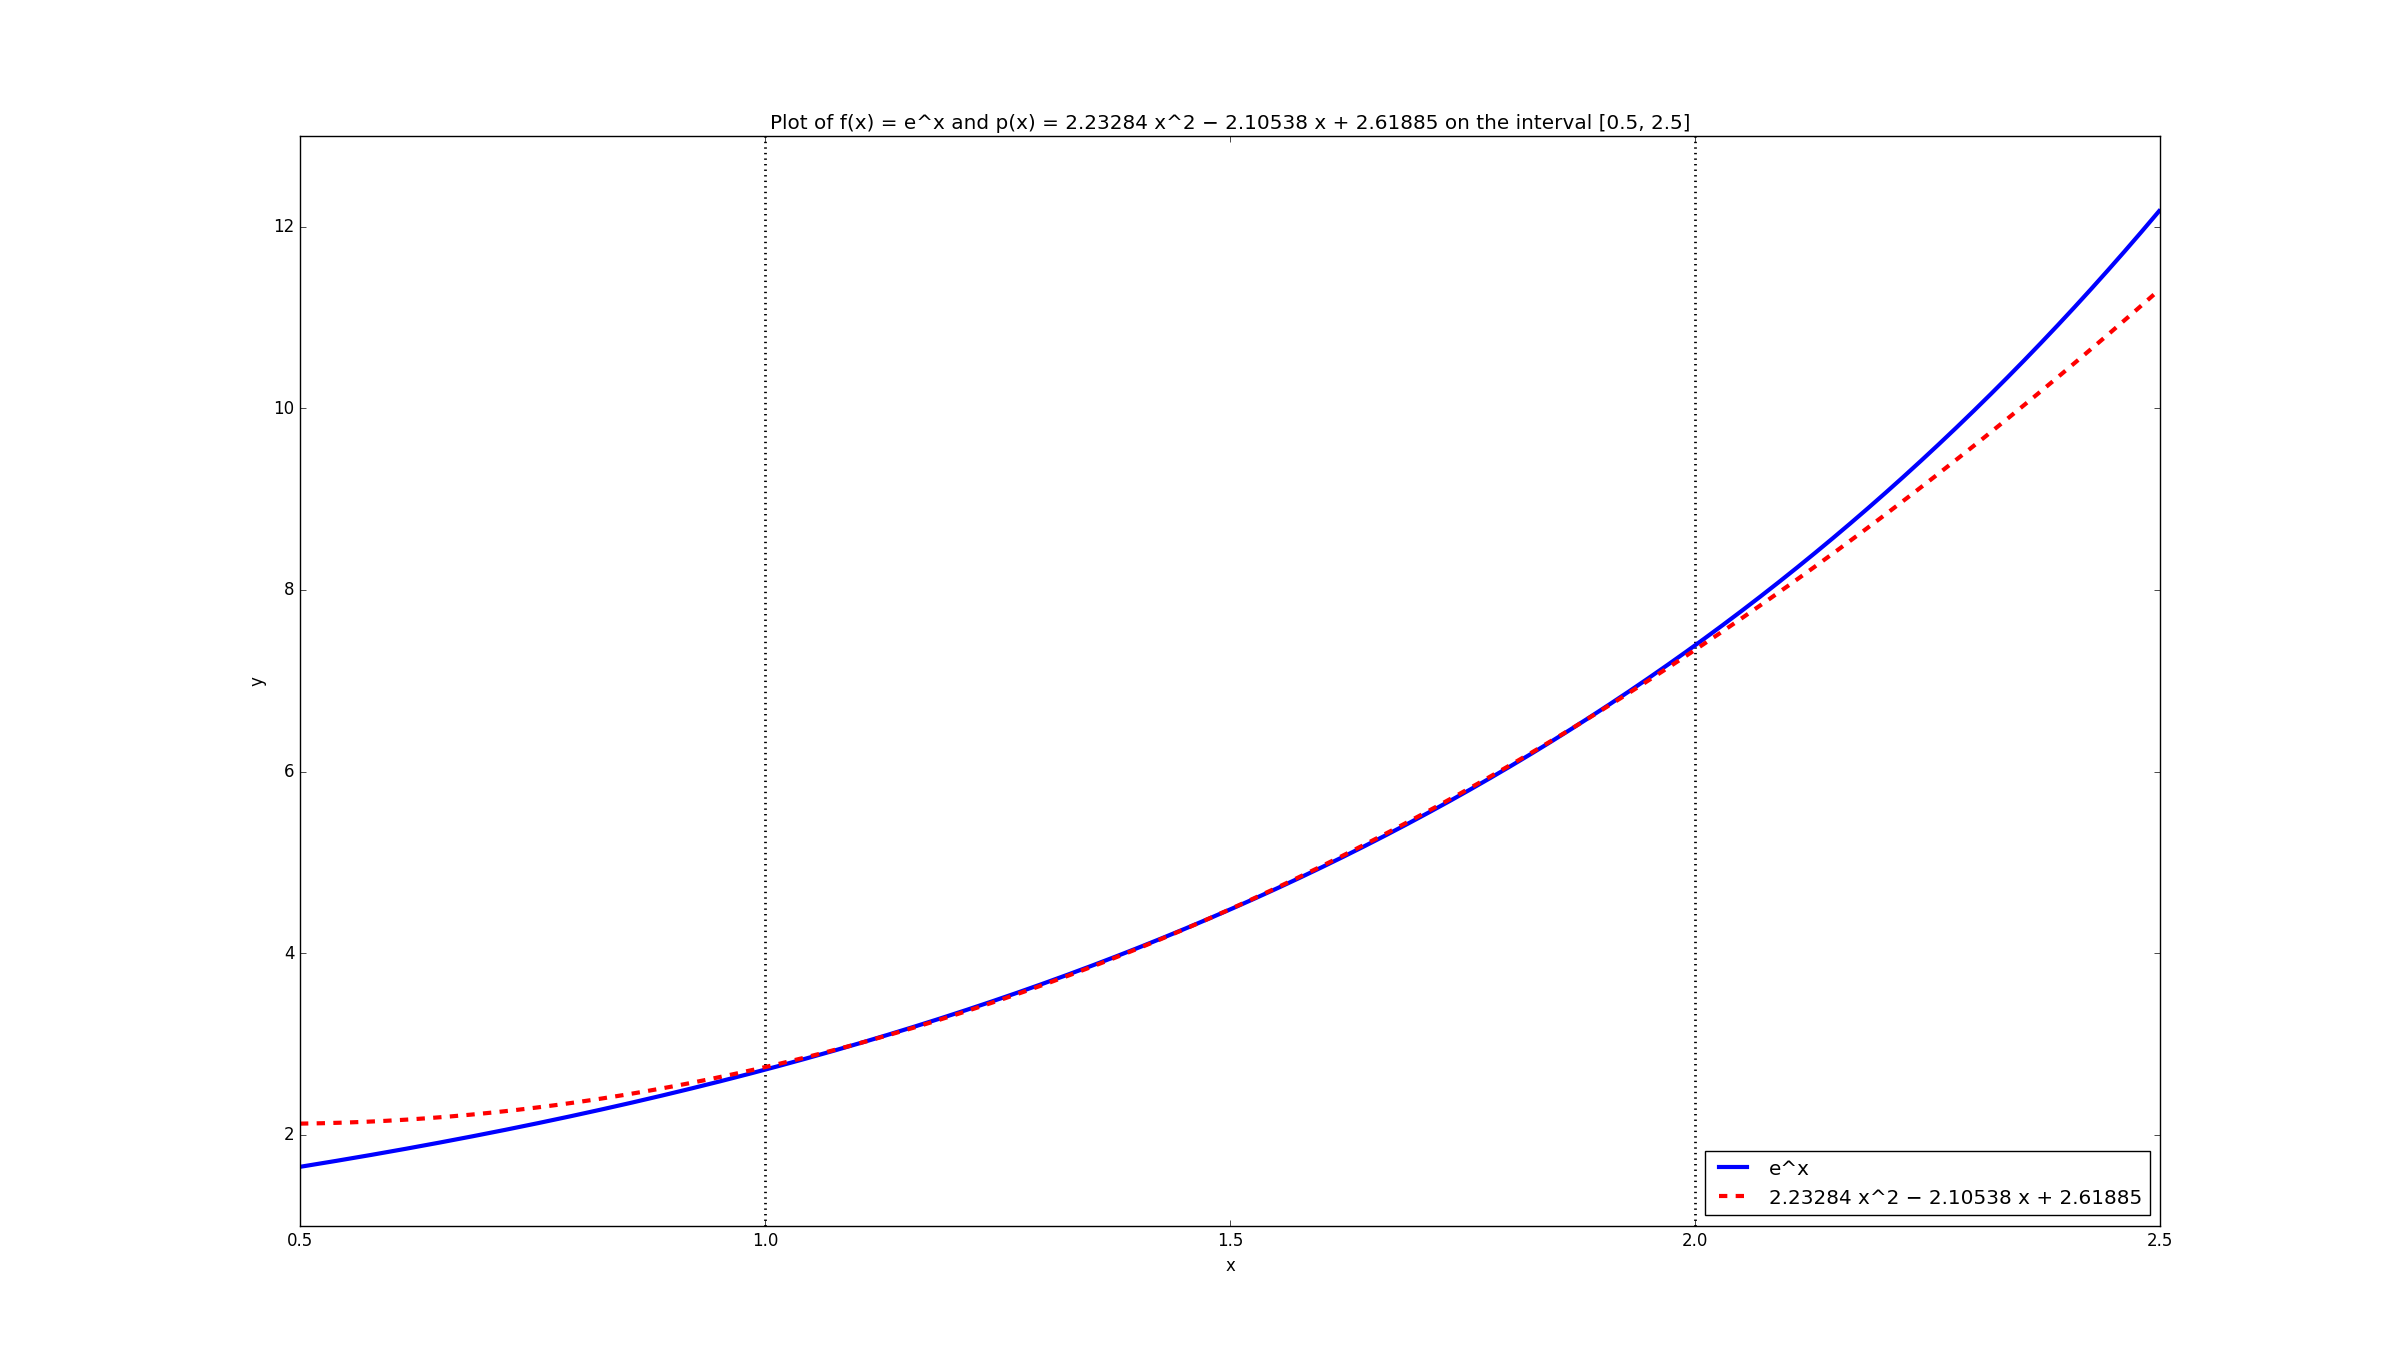
\includegraphics[trim={6cm, 0, 5cm, 2cm}, clip, width=\textwidth]{ortho_plot.png}
	\vspace{-10mm}
	\caption{Plot of $f(x) = e^x$ (solid line) and $p(x) = 2.23284 x^2 - 2.10538 x + 2.61885$ (dashed line), the polynomial constructed in 2 (a).}
	\label{Figure 1}
\end{figure}

% Stuff for wolfram alpha to simplify
(\frac{1}{4} n^2 + \frac{1}{4} n) (\frac{5}{4} n^2 + \frac{13}{4} n + \varepsilon) - n (\frac{5}{12} n^3 + \frac{9}{8} n^2 + \frac{17}{24} n + \delta)

(\frac{1}{4} n^2 + \frac{1}{4} n)^2 - n (\frac{1}{12} n^3 + \frac{1}{8} n^2 + \frac{1}{24} n)

% Incorrect work for #3
Hence $$\phi_0 (t) = \sqrt{1/2}, \ \ \ \phi_1 (t) = \sqrt{3/2} \ (t + 2), \ \ \ \text{and} \ \ \ \phi_2 (t) = \sqrt{5/8} \ (3t^2 + 12 t + 11).$$ Now by defining $f(t) = e^{t + 2}$ we have $$p_2 (t) = \langle f(t), \phi_0 \rangle \phi_0 + \langle f(t), \phi_1 \rangle \phi_1 + \langle f(t), \phi_2 \rangle \phi_2.$$ Since $$\langle f(t), \phi_0 \rangle = e^2 \sqrt{\frac{1}{2}} \int_{-1}^{1} e^t \approx 12.28050385,$$ $$\langle f(t), \phi_1 \rangle = e^2 \sqrt{\frac{3}{2}} \int_{-1}^{1} e^t (t + 2) = 2 e^3 \sqrt{\frac{3}{2}} \approx 49.19931667,$$ and $$\langle f(t), \phi_2 \rangle = e^2 \sqrt{\frac{5}{8}} \int_{-1}^{1} e^t (3t^2 + 12t + 11) = e^2 \left( 14 e - \frac{2}{e} \right) \sqrt{\frac{5}{8}} \approx 218.0081755$$ we have that 
\begin{align*}
p_2 (t) = 12.28050385 \sqrt{\frac{1}{2}} + 49.19931667 (t + 2) \sqrt{\frac{3}{2}} + 218.0081755 (3t^2 + 12 t + 11) \sqrt{\frac{5}{8}} \\
&= 
\end{align*}

% Some unused code
# Generate data set {(x_1, y_1), ..., (x_20, y_20)}
    for k in range(1, m + 1):
        # Initialize x_k = k/2
        x.append(k/2)

        # Initialize eps_k as a random number uniformly distributed in [-2, 2]
        epsilon = np.random.uniform(-2, 2)

        # Set y_k = 5x_k + 2 + eps_k
        y.append(5*k/2 + 2 + epsilon)
